% Full original method set. LightBSR corrected against official ICCV2025 Table 4.
% DEDBSR and all other baseline PSNR entries preserved from the archived full table.
\begin{table*}[!t]
\caption{B100 PSNR (dB) under nine anisotropic blur kernels and two noise levels for $\times4$ SR. Headers visualize the kernels in the order of LightBSR Table~4~\cite{yuan2025lightbsr}, which supplies the baseline scores. DEDBSR uses a separately trained anisotropic/noisy model. Bold/underline denote the best/second-best distinct scores, including ties.}
\label{tab:anisotropic}
\centering\footnotesize
\setlength{\tabcolsep}{4.5pt}
\renewcommand{\arraystretch}{1.03}
\begin{tabular}{clrrrrrrrrr}
\toprule
Noise & Method & \raisebox{-0.35\height}{
\includegraphics[height=0.25in]{figures/kernels/kernel_K1.png}} & \raisebox{-0.35\height}{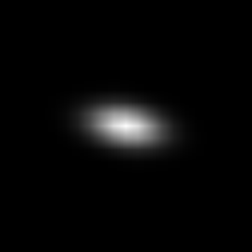
\includegraphics[height=0.25in]{figures/kernels/kernel_K2.png}} & \raisebox{-0.35\height}{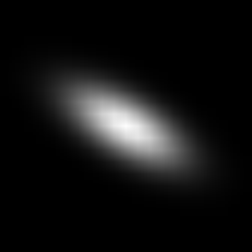
\includegraphics[height=0.25in]{figures/kernels/kernel_K3.png}} & \raisebox{-0.35\height}{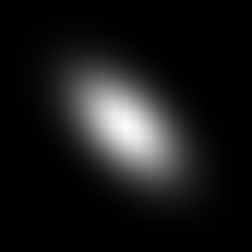
\includegraphics[height=0.25in]{figures/kernels/kernel_K4.png}} & \raisebox{-0.35\height}{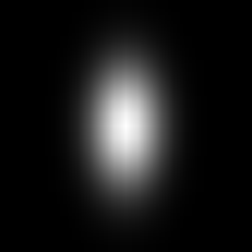
\includegraphics[height=0.25in]{figures/kernels/kernel_K5.png}} & \raisebox{-0.35\height}{
\includegraphics[height=0.25in]{figures/kernels/kernel_K6.png}} & \raisebox{-0.35\height}{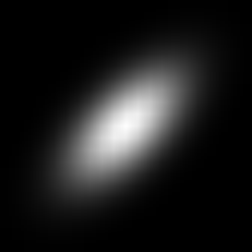
\includegraphics[height=0.25in]{figures/kernels/kernel_K7.png}} & \raisebox{-0.35\height}{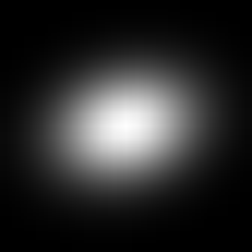
\includegraphics[height=0.25in]{figures/kernels/kernel_K8.png}} & \raisebox{-0.35\height}{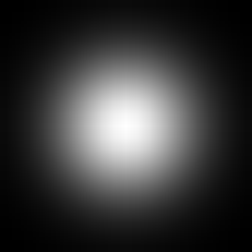
\includegraphics[height=0.25in]{figures/kernels/kernel_K9.png}}\\
\midrule
\multirow{9}{*}{5} & DnCNN+DAN & 26.18 & 26.14 & 24.89 & 24.64 & 24.61 & 24.52 & 24.37 & 24.01 & 23.63\\
 & DnCNN+DCLS & 26.15 & 26.12 & 24.89 & 24.66 & 24.62 & 24.52 & 24.39 & 24.03 & 23.65\\
 & DASR & 26.60 & 26.52 & 25.87 & 25.69 & 25.64 & 25.60 & 25.48 & 25.23 & 24.85\\
 & MRDA & 26.73 & 26.68 & 25.98 & 25.80 & 25.77 & 25.71 & 25.59 & 25.29 & 24.82\\
 & KDSR & 26.73 & 26.70 & 26.02 & 25.87 & 25.83 & 25.76 & 25.65 & 25.37 & 24.94\\
 & DSAT & 26.71 & 26.66 & 25.95 & 25.80 & 25.74 & 25.66 & 25.55 & 25.30 & 24.85\\
 & CDFormer-S & 26.77 & 26.69 & 26.00 & 25.85 & 25.82 & 25.75 & 25.64 & 25.34 & \second{24.97}\\
 & LightBSR & \second{26.82} & \second{26.76} & \second{26.06} & \second{25.91} & \second{25.87} & \second{25.81} & \second{25.70} & \best{25.41} & \best{25.05}\\
 & \textbf{DEDBSR} & \best{26.86} & \best{26.79} & \best{26.08} & \best{25.92} & \best{25.89} & \best{25.84} & \best{25.72} & \second{25.40} & \best{25.05}\\
\midrule
\multirow{9}{*}{10} & DnCNN+DAN & 25.69 & 25.63 & 24.62 & 24.42 & 24.39 & 24.29 & 24.18 & 23.89 & 23.54\\
 & DnCNN+DCLS & 25.67 & 25.62 & 24.62 & 24.43 & 24.40 & 24.29 & 24.19 & 23.91 & 23.56\\
 & DASR & 26.02 & 25.94 & 25.27 & 25.11 & 25.08 & 25.03 & 24.93 & 24.69 & 24.33\\
 & MRDA & 26.12 & 26.05 & 25.36 & 25.20 & 25.18 & 25.12 & 25.01 & 24.76 & 24.36\\
 & KDSR & 26.11 & 26.05 & 25.38 & 25.24 & 25.21 & 25.15 & 25.05 & 24.81 & \second{24.46}\\
 & DSAT & 26.07 & 26.04 & 25.29 & 25.18 & 25.14 & 25.09 & 24.97 & 24.72 & 24.36\\
 & CDFormer-S & 26.14 & 26.06 & 25.37 & 25.22 & 25.20 & 25.15 & 25.04 & 24.78 & 24.45\\
 & LightBSR & \second{26.18} & \second{26.10} & \second{25.41} & \second{25.27} & \second{25.24} & \second{25.19} & \second{25.08} & \second{24.83} & \best{24.53}\\
 & \textbf{DEDBSR} & \best{26.21} & \best{26.13} & \best{25.43} & \best{25.28} & \best{25.26} & \best{25.20} & \best{25.09} & \best{24.84} & \best{24.53}\\
\bottomrule
\end{tabular}
\end{table*}
